\documentclass{article}
\usepackage[utf8]{inputenc} % Required for inputting international characters
\usepackage[T1]{fontenc} % Output font encoding for international characters

%%%%%%%%%%%%%%%%%%%%%%%%%%%%%%%%%
% PACKAGE IMPORTS
%%%%%%%%%%%%%%%%%%%%%%%%%%%%%%%%%
\usepackage[tmargin=2cm,rmargin=1in,lmargin=1in,margin=0.85in,bmargin=2cm,footskip=.2in]{geometry}
\usepackage{amsmath,amsfonts,amsthm,amssymb,mathtools} %general maths stuff
\usepackage[varbb]{newpxmath} %maths tools
\usepackage{xfrac} %a/b fractions
\usepackage[makeroom]{cancel}
\usepackage{mathtools}
\usepackage{bookmark}
\usepackage{enumitem}
\usepackage{hyperref,theoremref}
\hypersetup{
	pdftitle={Past Paper},
	colorlinks=true, linkcolor=black!90,
	bookmarksnumbered=true,
	bookmarksopen=true
}
\usepackage[most,many,breakable]{tcolorbox}
\usepackage{xcolor}
\usepackage{varwidth}
\usepackage{varwidth}
\usepackage{etoolbox}
\usepackage{nameref}
\usepackage{multicol,array}
\usepackage{tikz-cd}
\usepackage[ruled,vlined,linesnumbered]{algorithm2e}
\usepackage{comment} % enables the use of multi-line comments (\ifx \fi) 
\usepackage{import}
\usepackage{xifthen}
\usepackage{pdfpages}
\usepackage{transparent}
\usepackage{tikzsymbols}

\usepackage[default]{raleway}
\usepackage{sectsty}
\renewcommand*\familydefault{\sfdefault} % Force the sans-serif version of any font used
\allsectionsfont{\sffamily\mdseries\upshape} % (See the fntguide.pdf for font help)

\usepackage[nottoc,notlof,notlot]{tocbibind} % Put the bibliography in the ToC
\usepackage[titles,subfigure]{tocloft} % Alter the style of the Table of Contents
\renewcommand{\cftsecfont}{\rmfamily\mdseries\upshape}
\renewcommand{\cftsecpagefont}{\rmfamily\mdseries\upshape} % No bold!

\usepackage{calc}
\usepackage{subfig}
\usepackage{pgfplots}
\pgfplotsset{compat = newest}


%%%%%%%%%%%%%%%%%%%%%%%%%%%%%%J
% SELF MADE COLORS
%%%%%%%%%%%%%%%%%%%%%%%%%%%%%%

\definecolor{myg}{RGB}{56, 140, 70}
\definecolor{myb}{RGB}{45, 111, 177}
\definecolor{myr}{RGB}{199, 68, 64}
\definecolor{mytheorembg}{HTML}{F2F2F9}
\definecolor{mytheoremfr}{HTML}{00007B}
\definecolor{mylenmabg}{HTML}{FFFAF8}
\definecolor{mylenmafr}{HTML}{983b0f}
\definecolor{mypropbg}{HTML}{f2fbfc}
\definecolor{mypropfr}{HTML}{191971}
\definecolor{myexamplebg}{HTML}{F2FBF8}
\definecolor{myexamplefr}{HTML}{88D6D1}
\definecolor{myexampleti}{HTML}{2A7F7F}
\definecolor{mydefinitbg}{HTML}{E5E5FF}
\definecolor{mydefinitfr}{HTML}{3F3FA3}
\definecolor{notesgreen}{RGB}{0,162,0}
\definecolor{myp}{RGB}{197, 92, 212}
\definecolor{mygr}{HTML}{2C3338}
\definecolor{myred}{RGB}{127,0,0}
\definecolor{myyellow}{RGB}{169,121,69}
\definecolor{myexercisebg}{HTML}{F2FBF8}
\definecolor{myexercisefg}{HTML}{88D6D1}


%%%%%%%%%%%%%%%%%%%%%%%%%%%%
% TCOLORBOX SETUPS
%%%%%%%%%%%%%%%%%%%%%%%%%%%%
%================================
% EXAMPLE BOX
%================================

\newtcbtheorem[number within=section]{Example}{Example}
{%
	colback = myexamplebg
	,breakable
	,colframe = myexamplefr
	,coltitle = myexampleti
	,boxrule = 1pt
	,sharp corners
	,detach title
	,before upper=\tcbtitle\par\smallskip
	,fonttitle = \bfseries
	,description font = \mdseries
	,separator sign none
	,description delimiters parenthesis
}
{ex}

%================================
% Question BOX
%================================

\makeatletter
\newtcbtheorem{question}{Question}{enhanced,
	breakable,
	colback=gray!20!white,
	colframe=mygr,
	attach boxed title to top left={yshift*=-\tcboxedtitleheight},
	fonttitle=\bfseries,
	title={#2},
	boxed title size=title,
	boxed title style={%
		sharp corners,
		rounded corners=northwest,
		colback=tcbcolframe,
		boxrule=0pt,
	},
	underlay boxed title={%
		\path[fill=tcbcolframe] (title.south west)--(title.south east)
		to[out=0, in=180] ([xshift=5mm]title.east)--
		(title.center-|frame.east)
		[rounded corners=\kvtcb@arc] |-
		(frame.north) -| cycle;
	},
	#1
}{def}
\makeatother


%================================
% NOTE BOX
%================================


\usetikzlibrary{arrows,calc,shadows.blur}
\tcbuselibrary{skins}
\newtcolorbox{questionpart}[2][]{%
	enhanced jigsaw,
	colback=white,
	colframe=gray!80!black,
	size=small,
	boxrule=1pt,
	title=\textit{#2},
	halign title=flush center,
	coltitle=black,
	breakable,
	drop shadow=black!50!white,
	attach boxed title to top left={xshift=0.2cm,yshift=-\tcboxedtitleheight/2,yshifttext=-\tcboxedtitleheight/2},
	minipage boxed title=0.5cm,
	boxed title style={%
		colback=white,
		size=fbox,
		boxrule=1pt,
		boxsep=2pt,
		underlay={%
			\coordinate (dotA) at ($(interior.west) + (-0.5pt,0)$);
			\coordinate (dotB) at ($(interior.east) + (0.5pt,0)$);
			\begin{scope}
				\clip (interior.north west) rectangle ([xshift=3ex]interior.east);
				\filldraw [white, blur shadow={shadow opacity=60, shadow yshift=-.75ex}, rounded corners=2pt] (interior.north west) rectangle (interior.south east);
			\end{scope}
			\begin{scope}[gray!80!black]
				\fill (dotA) circle (2pt);
				\fill (dotB) circle (2pt);
			\end{scope}
		},
	},
	#1,
}

%%%%%%%%%%%%%%%%%%%%%%%%%%%%%%
% SELF MADE COMMANDS
%%%%%%%%%%%%%%%%%%%%%%%%%%%%%%

\newcommand{\qs}[1]{\begin{question}{}{}#1\end{question}}
\newcommand{\qsp}[2]{\begin{questionpart}{#1}{}#2\end{questionpart}}

\newcommand{\plotbasic}[3][black]{ % colour func formatted
		\begin{tikzpicture}
		\begin{axis}[
				axis lines = center,
				xlabel = \(x\),
				ylabel = \(f(x)\),
			]
			
			\addplot [
				domain=-5:5, 
				samples=100, 
				color={#1},
			]
			{#2};
			\addlegendentry{#3}
		\end{axis}
	\end{tikzpicture}
}
\newenvironment{plotter}{
	\begin{tikzpicture}
		\begin{axis}[
			axis lines = center,
			xlabel = \(x\),
			ylabel = \(f(x)\),
		]
}
{
\end{axis}
\end{tikzpicture}
}


\newenvironment{unitcircled}{
\usetikzlibrary {intersections}
\begin{tikzpicture}[scale=2]
	\draw[step=.5cm,gray,very thin] (-1.2,-1.2) grid (1.2,1.2);
	\draw[->] (-1.2,0) -- (1.2,0) coordinate (x axis);
	\draw[->] (0,-1.2) -- (0,1.2) coordinate (y axis);
	\draw (0,0) circle [radius=1cm];
	
	\foreach \x/\xtext in {-1, -0.5/-\frac{1}{2}, 0, 0.5/\frac{1}{2}, 1}
	\draw (\x cm,1pt) -- (\x cm,-1pt) node[anchor=north,fill=white] {$\xtext$};
	\foreach \y/\ytext in {-1, -0.5/-\frac{1}{2}, 0.5/\frac{1}{2}, 1}
	\draw (1pt,\y cm) -- (-1pt,\y cm) node[anchor=east,fill=white] {$\ytext$};
} {
\end{tikzpicture}
}

\newcommand*\circled[1]{\tikz[baseline=(char.base)]{
	\node[shape=circle,draw,inner sep=1pt] (char) {#1};}}
\newcommand\getcurrentref[1]{%
\ifnumequal{\value{#1}}{0}
{??}
{\the\value{#1}}%
}
\newcommand{\getCurrentSectionNumber}{\getcurrentref{section}}


\newcounter{mylabelcounter}

\makeatletter
\newcommand{\setword}[2]{%
\phantomsection
#1\def\@currentlabel{\unexpanded{#1}}\label{#2}%
}
\makeatother

\tikzset{
symbol/.style={
	draw=none,
	every to/.append style={
		edge node={node [sloped, allow upside down, auto=false]{$#1$}}}
}
}


%%%%%%%%%%%%%%%%%%%%%%%%%%%%%%%%%%%%%%%%%%%
% TABLE OF CONTENTS
%%%%%%%%%%%%%%%%%%%%%%%%%%%%%%%%%%%%%%%%%%%

\usepackage{tikz}
\definecolor{doc}{RGB}{0,60,110}
\usepackage{titletoc}
\contentsmargin{0cm}
\titlecontents{chapter}[3.7pc]
{\addvspace{30pt}%
	\begin{tikzpicture}[remember picture, overlay]%
		\draw[fill=doc!60,draw=doc!60] (-7,-.1) rectangle (-0.9,.5);%
		\pgftext[left,x=-3.5cm,y=0.2cm]{\color{white}\Large\sc\bfseries Chapter\ \thecontentslabel};%
	\end{tikzpicture}\color{doc!60}\large\sc\bfseries}%
{}
{}
{\;\titlerule\;\large\sc\bfseries Page \thecontentspage
	\begin{tikzpicture}[remember picture, overlay]
		\draw[fill=doc!60,draw=doc!60] (2pt,0) rectangle (4,0.1pt);
\end{tikzpicture}}%
\titlecontents{section}[3.7pc]
{\addvspace{2pt}}
{\contentslabel[\thecontentslabel]{2pc}}
{}
{\hfill\small \thecontentspage}
[]
\titlecontents*{subsection}[3.7pc]
{\addvspace{-1pt}\small}
{}
{}
{\ --- \small\thecontentspage}
[ \textbullet\ ][]

\makeatletter
\renewcommand{\tableofcontents}{%
	\chapter*{%
		\vspace*{-20\p@}%
		\begin{tikzpicture}[remember picture, overlay]%
			\pgftext[right,x=15cm,y=0.2cm]{\color{doc!60}\Huge\sc\bfseries \contentsname};%
			\draw[fill=doc!60,draw=doc!60] (13,-.75) rectangle (20,1);%
			\clip (13,-.75) rectangle (20,1);
			\pgftext[right,x=15cm,y=0.2cm]{\color{white}\Huge\sc\bfseries \contentsname};%
	\end{tikzpicture}}%
	\@starttoc{toc}}
\makeatother
%Symbols
\newcommand{\dg}{^\circ}
\newcommand{\dang}{\measuredangle} %% Directed angle
\newcommand{\lm}{\lambda}
\newcommand{\uin}{\mathbin{\rotatebox[origin=c]{90}{$\in$}}}
\newcommand{\usubset}{\mathbin{\rotatebox[origin=c]{90}{$\subset$}}}

%Shortcuts
\newcommand{\ii}{\item}
\newcommand{\lthen}{\rightarrow}
\newcommand{\opname}{\operatorname}

%Diff/Int
\newcommand{\differen}[1][y]{\frac{\Delta #1}{\Delta x}}
\newcommand{\differend}[1][y]{\dfrac{\Delta #1}{\Delta x}}
\newcommand{\twodifferen}[1][y]{\frac{\Delta^2 #1}{\Delta x^2}}
\newcommand{\twodifferend}[1][y]{\dfrac{\Delta^2 #1}{\Delta x^2}}
\newcommand{\limit}[2]{\lim\limits_{#1 \to #2}}
\newcommand{\integratestart}[4][x]{\int_{#3}^{#4} \left( {#2} \right) d{#1}} %x/t/etc func lowerlim upperlim
\newcommand{\integrateinner}[3]{\left[ {#1} \right]_{#2}^{#3}} % func lowerlim upperlim

\DeclareMathOperator{\cosec}{cosec}
\DeclareMathOperator{\ud}{\textit{undefined}}

\newcommand{\func}[2][f]{#1 \left( #2 \right)}


%---------------------------------------
% BlackBoard Math Fonts :-
%---------------------------------------

%Captital Letters
\newcommand{\bbA}{\mathbb{A}}	\newcommand{\bbB}{\mathbb{B}}
\newcommand{\bbC}{\mathbb{C}}	\newcommand{\bbD}{\mathbb{D}}
\newcommand{\bbE}{\mathbb{E}}	\newcommand{\bbF}{\mathbb{F}}
\newcommand{\bbG}{\mathbb{G}}	\newcommand{\bbH}{\mathbb{H}}
\newcommand{\bbI}{\mathbb{I}}	\newcommand{\bbJ}{\mathbb{J}}
\newcommand{\bbK}{\mathbb{K}}	\newcommand{\bbL}{\mathbb{L}}
\newcommand{\bbM}{\mathbb{M}}	\newcommand{\bbN}{\mathbb{N}}
\newcommand{\bbO}{\mathbb{O}}	\newcommand{\bbP}{\mathbb{P}}
\newcommand{\bbQ}{\mathbb{Q}}	\newcommand{\bbR}{\mathbb{R}}
\newcommand{\bbS}{\mathbb{S}}	\newcommand{\bbT}{\mathbb{T}}
\newcommand{\bbU}{\mathbb{U}}	\newcommand{\bbV}{\mathbb{V}}
\newcommand{\bbW}{\mathbb{W}}	\newcommand{\bbX}{\mathbb{X}}
\newcommand{\bbY}{\mathbb{Y}}	\newcommand{\bbZ}{\mathbb{Z}}

%---------------------------------------
% MathCal Fonts :-
%---------------------------------------

%Captital Letters
\newcommand{\mcA}{\mathcal{A}}	\newcommand{\mcB}{\mathcal{B}}
\newcommand{\mcC}{\mathcal{C}}	\newcommand{\mcD}{\mathcal{D}}
\newcommand{\mcE}{\mathcal{E}}	\newcommand{\mcF}{\mathcal{F}}
\newcommand{\mcG}{\mathcal{G}}	\newcommand{\mcH}{\mathcal{H}}
\newcommand{\mcI}{\mathcal{I}}	\newcommand{\mcJ}{\mathcal{J}}
\newcommand{\mcK}{\mathcal{K}}	\newcommand{\mcL}{\mathcal{L}}
\newcommand{\mcM}{\mathcal{M}}	\newcommand{\mcN}{\mathcal{N}}
\newcommand{\mcO}{\mathcal{O}}	\newcommand{\mcP}{\mathcal{P}}
\newcommand{\mcQ}{\mathcal{Q}}	\newcommand{\mcR}{\mathcal{R}}
\newcommand{\mcS}{\mathcal{S}}	\newcommand{\mcT}{\mathcal{T}}
\newcommand{\mcU}{\mathcal{U}}	\newcommand{\mcV}{\mathcal{V}}
\newcommand{\mcW}{\mathcal{W}}	\newcommand{\mcX}{\mathcal{X}}
\newcommand{\mcY}{\mathcal{Y}}	\newcommand{\mcZ}{\mathcal{Z}}


%---------------------------------------
% Bold Math Fonts :-
%---------------------------------------

%Captital Letters
\newcommand{\bmA}{\boldsymbol{A}}	\newcommand{\bmB}{\boldsymbol{B}}
\newcommand{\bmC}{\boldsymbol{C}}	\newcommand{\bmD}{\boldsymbol{D}}
\newcommand{\bmE}{\boldsymbol{E}}	\newcommand{\bmF}{\boldsymbol{F}}
\newcommand{\bmG}{\boldsymbol{G}}	\newcommand{\bmH}{\boldsymbol{H}}
\newcommand{\bmI}{\boldsymbol{I}}	\newcommand{\bmJ}{\boldsymbol{J}}
\newcommand{\bmK}{\boldsymbol{K}}	\newcommand{\bmL}{\boldsymbol{L}}
\newcommand{\bmM}{\boldsymbol{M}}	\newcommand{\bmN}{\boldsymbol{N}}
\newcommand{\bmO}{\boldsymbol{O}}	\newcommand{\bmP}{\boldsymbol{P}}
\newcommand{\bmQ}{\boldsymbol{Q}}	\newcommand{\bmR}{\boldsymbol{R}}
\newcommand{\bmS}{\boldsymbol{S}}	\newcommand{\bmT}{\boldsymbol{T}}
\newcommand{\bmU}{\boldsymbol{U}}	\newcommand{\bmV}{\boldsymbol{V}}
\newcommand{\bmW}{\boldsymbol{W}}	\newcommand{\bmX}{\boldsymbol{X}}
\newcommand{\bmY}{\boldsymbol{Y}}	\newcommand{\bmZ}{\boldsymbol{Z}}
%Small Letters
\newcommand{\bma}{\boldsymbol{a}}	\newcommand{\bmb}{\boldsymbol{b}}
\newcommand{\bmc}{\boldsymbol{c}}	\newcommand{\bmd}{\boldsymbol{d}}
\newcommand{\bme}{\boldsymbol{e}}	\newcommand{\bmf}{\boldsymbol{f}}
\newcommand{\bmg}{\boldsymbol{g}}	\newcommand{\bmh}{\boldsymbol{h}}
\newcommand{\bmi}{\boldsymbol{i}}	\newcommand{\bmj}{\boldsymbol{j}}
\newcommand{\bmk}{\boldsymbol{k}}	\newcommand{\bml}{\boldsymbol{l}}
\newcommand{\bmm}{\boldsymbol{m}}	\newcommand{\bmn}{\boldsymbol{n}}
\newcommand{\bmo}{\boldsymbol{o}}	\newcommand{\bmp}{\boldsymbol{p}}
\newcommand{\bmq}{\boldsymbol{q}}	\newcommand{\bmr}{\boldsymbol{r}}
\newcommand{\bms}{\boldsymbol{s}}	\newcommand{\bmt}{\boldsymbol{t}}
\newcommand{\bmu}{\boldsymbol{u}}	\newcommand{\bmv}{\boldsymbol{v}}
\newcommand{\bmw}{\boldsymbol{w}}	\newcommand{\bmx}{\boldsymbol{x}}
\newcommand{\bmy}{\boldsymbol{y}}	\newcommand{\bmz}{\boldsymbol{z}}

\graphicspath{{./images/}}

\title{\huge{C3 X}}
\author{\huge{Jack Maguire}}
\date{}

\begin{document}

\maketitle


\qs{
\qsp{a}{
	\[ y = \frac{x^2 - 6x + 12}{4x - 11} \]
	\begin{multicols}{2}
		\noindent
		\begin{align*}
			v &= 4x - 11 \\
			v^\prime &= 4 
		\end{align*}
		\pagebreak
		\begin{align*}
			u &= x^2 - 6x + 12 \\
			u^\prime &= 2x - 6
		\end{align*}
	\end{multicols}
	\noindent
	\begin{align*}
		\differen &= \frac{vu^\prime - v^\prime u}{v^2} \\
				  &= \frac{(4x-11)(2x-6) - 4(x^2-6x+12)}{(4x-11)^2} \\
				  &= \frac{8x^2 -46x + 66 - 4x^2 + 24x - 48}{(4x-11)^2} \\
				  &= \frac{4x^2 -22x + 18}{(4x-11)^2} \\
				  &= \frac{4x^2 -22x + 18}{16x^2 - 88x + 121} \\
	\end{align*}
}
\qsp{b}{
	\(y\) is decreasing \(\therefore \differen < 0\)
	
	\[ \frac{4x^2 -22x + 18}{16x^2 - 88x + 121} < 0 \]
	Since \( 16x^2 - 88x + 121 \) only has one repeated root, and is a positive curve, it will never go below zero, so we can ignore solutions from it.
	
	\begin{align*}
		 \frac{4x^2 -22x + 18}{16x^2 - 88x + 121} &< 0 \\
		 4x^2 -22x + 18 &< 0 \\
		 (2x-1)(4x-9) &< 0 \\
		 1 < x < 4.5 &
	\end{align*}
}
}

\qs{
\begin{align*}
	\sin 2\theta &= \cot \theta \\
	2\sin \theta \cos \theta &= \frac{\cos \theta}{\sin \theta} \\
	2\sin ^2 \theta \cos \theta &= \cos \theta \\
	2\sin ^2 \theta \cos \theta - \cos \theta &= 0\\
	\left( \cos \theta \right) \left(  2\sin ^2 \theta - 1  \right) &= 0
\end{align*}
\begin{multicols}{2}
	\noindent
	\begin{align*}
		\cos \theta &= 0 \\
		\theta &= 90 \dg
	\end{align*}
	\columnbreak
	\begin{align*}
		 2\sin ^2 \theta - 1 &= 0 \\
		 \sin ^2 \theta &= \frac{1}{2} \\
		 \sin \theta &= \pm \frac{\sqrt{2}}{2} \\
		 \theta &= 45 \dg, 135 \dg
	\end{align*}
\end{multicols}
\[ \theta = 45 \dg, 90 \dg, 135 \dg \]
}

\qs{
\qsp{a}{
	\begin{align*}
		&= \func{1 + \sqrt{9}} \\
		&= \func{4} \\
		&= 1 + \sqrt{4} \\
		&= 3
	\end{align*}
}
\qsp{b}{
	\begin{align*}
		y &= 1 + \sqrt{x} \\
		x &= 1 + \sqrt{y} \\
		x - 1 &= \sqrt{y} \\
		(x-1)^2 &= y \\
		\func{x} &= (x-1)^2
	\end{align*}
}
\qsp{c}{
	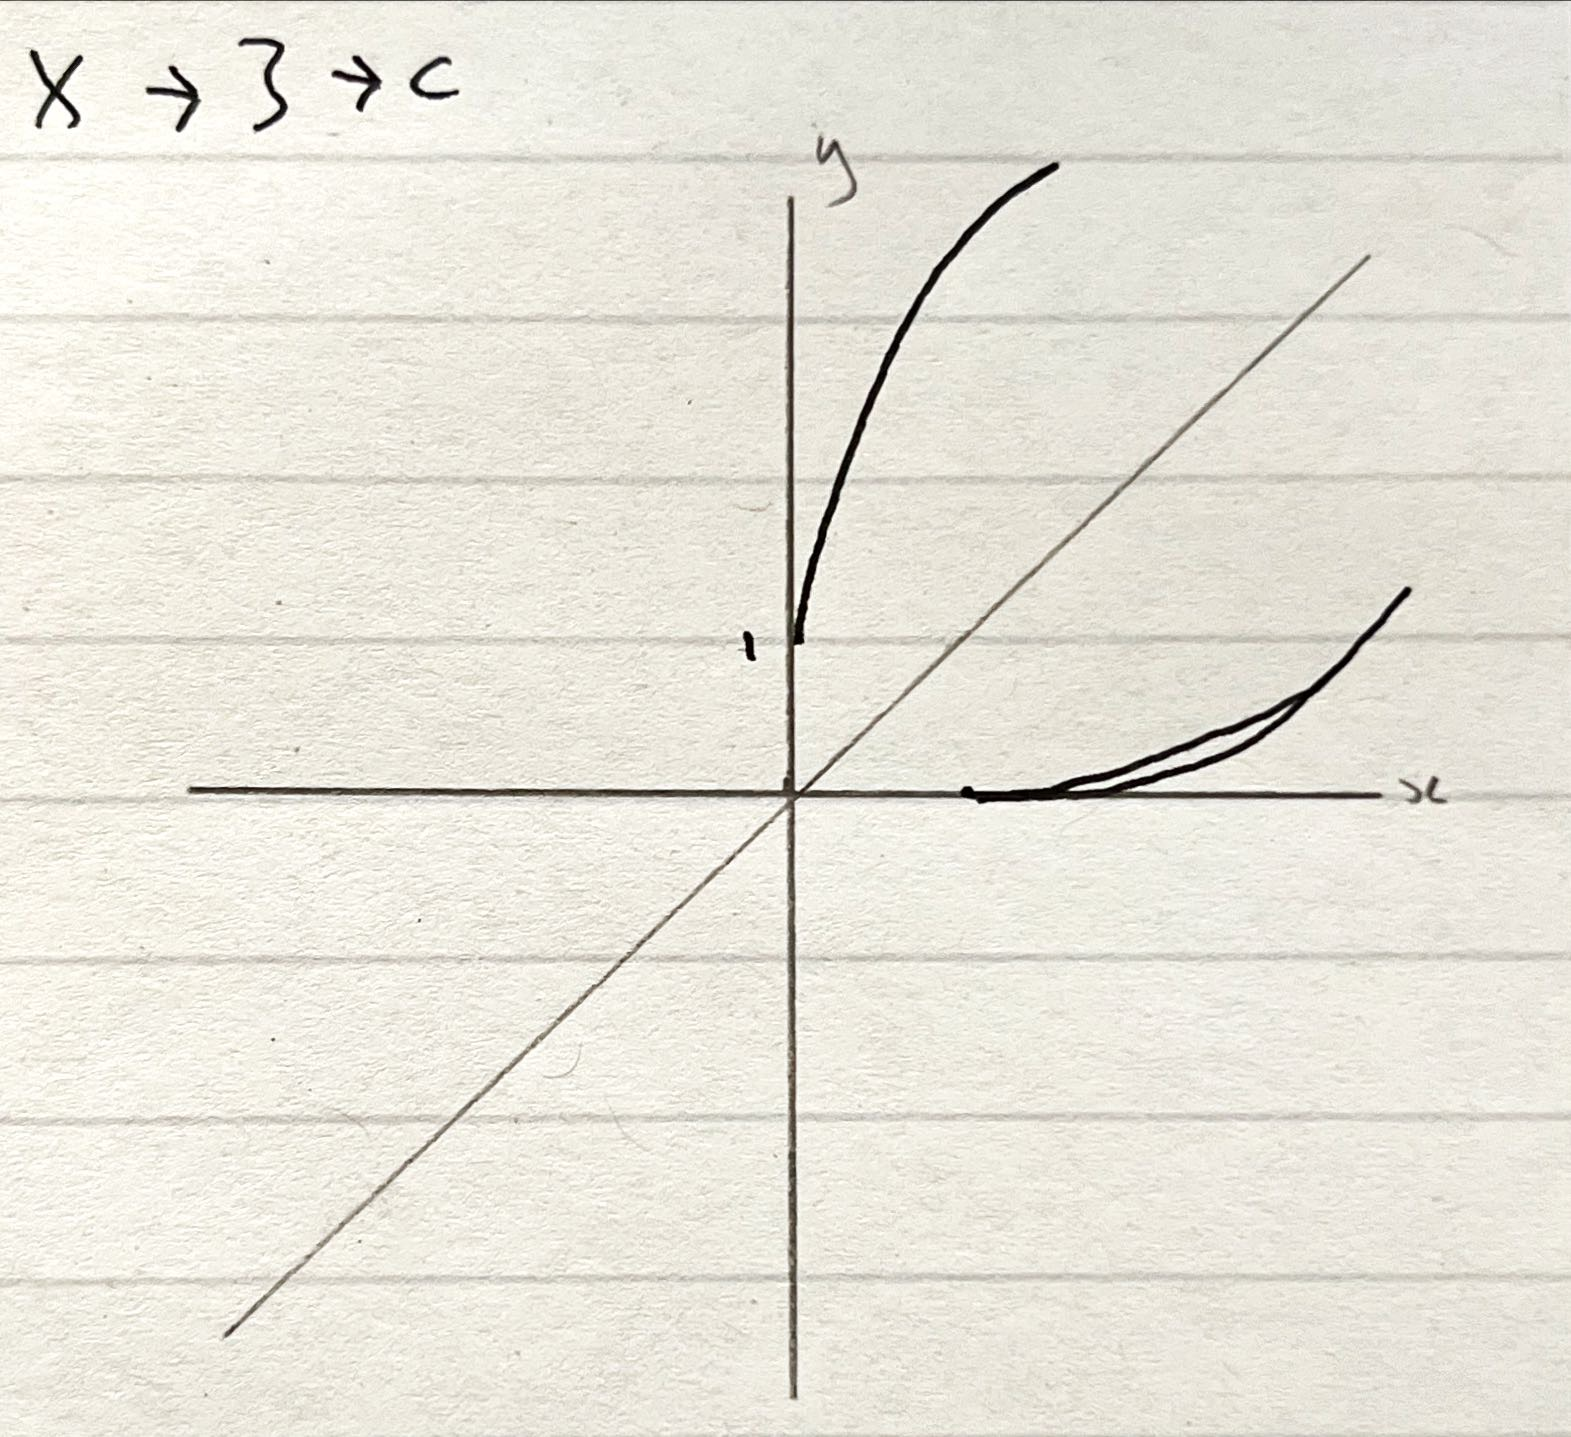
\includegraphics[width=\textwidth / 3]{x3c}
}
\qsp{d}{
	\begin{align*}
		1 + \sqrt{x} &= (x-1)^2 \\
		\sqrt{x} &= x^2 - 2x \\
		x &= \left( x^2 - 2x \right) ^2 \\
		0 &= x^4 - 4x^3 + 4x^2 - x
	\end{align*}
	We could say that \(x = 0\), but we can see it is invalid on the graph and ignore it.
	\begin{align*}
		\func{x} &= x^3 - 4x^2 + 4x - 1 \\
		\func{1} &= 1 - 4 + 4 - 1 = 0 \\
		0 &= (x-1)(x^2 + bx + 1) \\ 
		0 &= \ldots - x^2 + bx^2 + \ldots \\
		-1 + b &= -4 \\
		b &= -3 \\
		\func{x} &= (x-1)(x^2-3x+1)
	\end{align*}
	We could say that \(x = 1\), but we can see it is invalid on the graph and ignore it.
	\begin{align*}
		0 &= x^2 - 3x + 1 \\
		x &= \frac{-b \pm \sqrt{b^2-4ac}}{2a} \\
		&= \frac{3 \pm \sqrt{9 - 4}}{2} \\
	\end{align*}
	We could say that \(x = \frac{3 - \sqrt{5}}{2}\), but we can see it is invalid on the graph and ignore it.
	\[ x = \frac{3 + \sqrt{5}}{2} \]
}
}

\qs{
\qsp{a}{
	\begin{align*}
		\frac{\Delta y}{\Delta x} &= \frac{3y^2 - 4}{y^3-4y} \\
		\differen &= \frac{y^3-4y}{3y^2-4} \\
		2 &= \frac{3y^2-4}{y^3-4y} \\
		1 &= \frac{3y^2-4}{2y^3-8y} \\
		2y^3-8y &= 3y^2-4
		y &= \frac{3y^2-4}{2y^2-8} \\
		???
	\end{align*}
}
\qsp{b}{
	???
}
}

\qs{
\begin{align*}
	\differen &= (-1) \left(4e^{2-x}\right)-(-2) \left(e^{4-2x}\right) \\
			  &= -4e^{2-x} + 2e^{4-2x} \\
	0 &= -4e^{2-x} + 2e^{4-2x} \\
	2e^{2-x} &= e^{4-2x} \\
	2e^{2-x} &= \left( e^{4-2x} \right) ^2 \\ \\
	\text{Let } y &= e^{2-x} \\
	2y &= y^2 \\
	0 &= y^2 - 2y \\
	y &= 0, 2 \\
	\ln{0} &\nequiv \bbR \\
	e^{2-x} &= 2 \\
	x &= 2 - \ln{2} \\
	&= 1.307 \\ \\
	y &= 4e^{2-x} - e^{4-2x} \\
	&= 4 \\ \\
	\differen_{1.25} &= 0.49 \\
	\differen_{1.307} &= 0 \\
	\differen_{1.35} &= -0.32 \\
\end{align*}
\begin{itemize}
	\ii Stationary Point = \((1.307, 4)\)
	\ii Kind = Maximum
\end{itemize}
}

\qs{
\qsp{a}{
	???
}
\qsp{b}{
	\begin{align*}
		R \cos \left( \theta - \alpha \right) &= R\cos \theta \cos \alpha + R\sin \theta \sin \alpha \\
		\\
		R \sin \alpha &= 2 \\
		R \cos \alpha &= 5 \\
		\tan \alpha &= \frac{2}{5} \\
		\alpha &= 21.8 \\
		\\
		R^2 &= 5^2 + 2^2 \\
		R &= \sqrt{25 + 4} \\
		R &= \sqrt{29} \\
		\\
		5\cos \theta + 2\sin \theta &\equiv \sqrt{29} \cos \left( \theta - 21.8 \dg \right)
	\end{align*}
}
\qsp{c}{
	???
}
}

\qs{
\qsp{a}{
\begin{enumerate}
	\ii Take the natural logarithm of x value.
	\ii Shift the graph right by 12 units.
	\ii Shrink the graph horizontally by a factor of 4.
\end{enumerate}
}
\qsp{b}{
	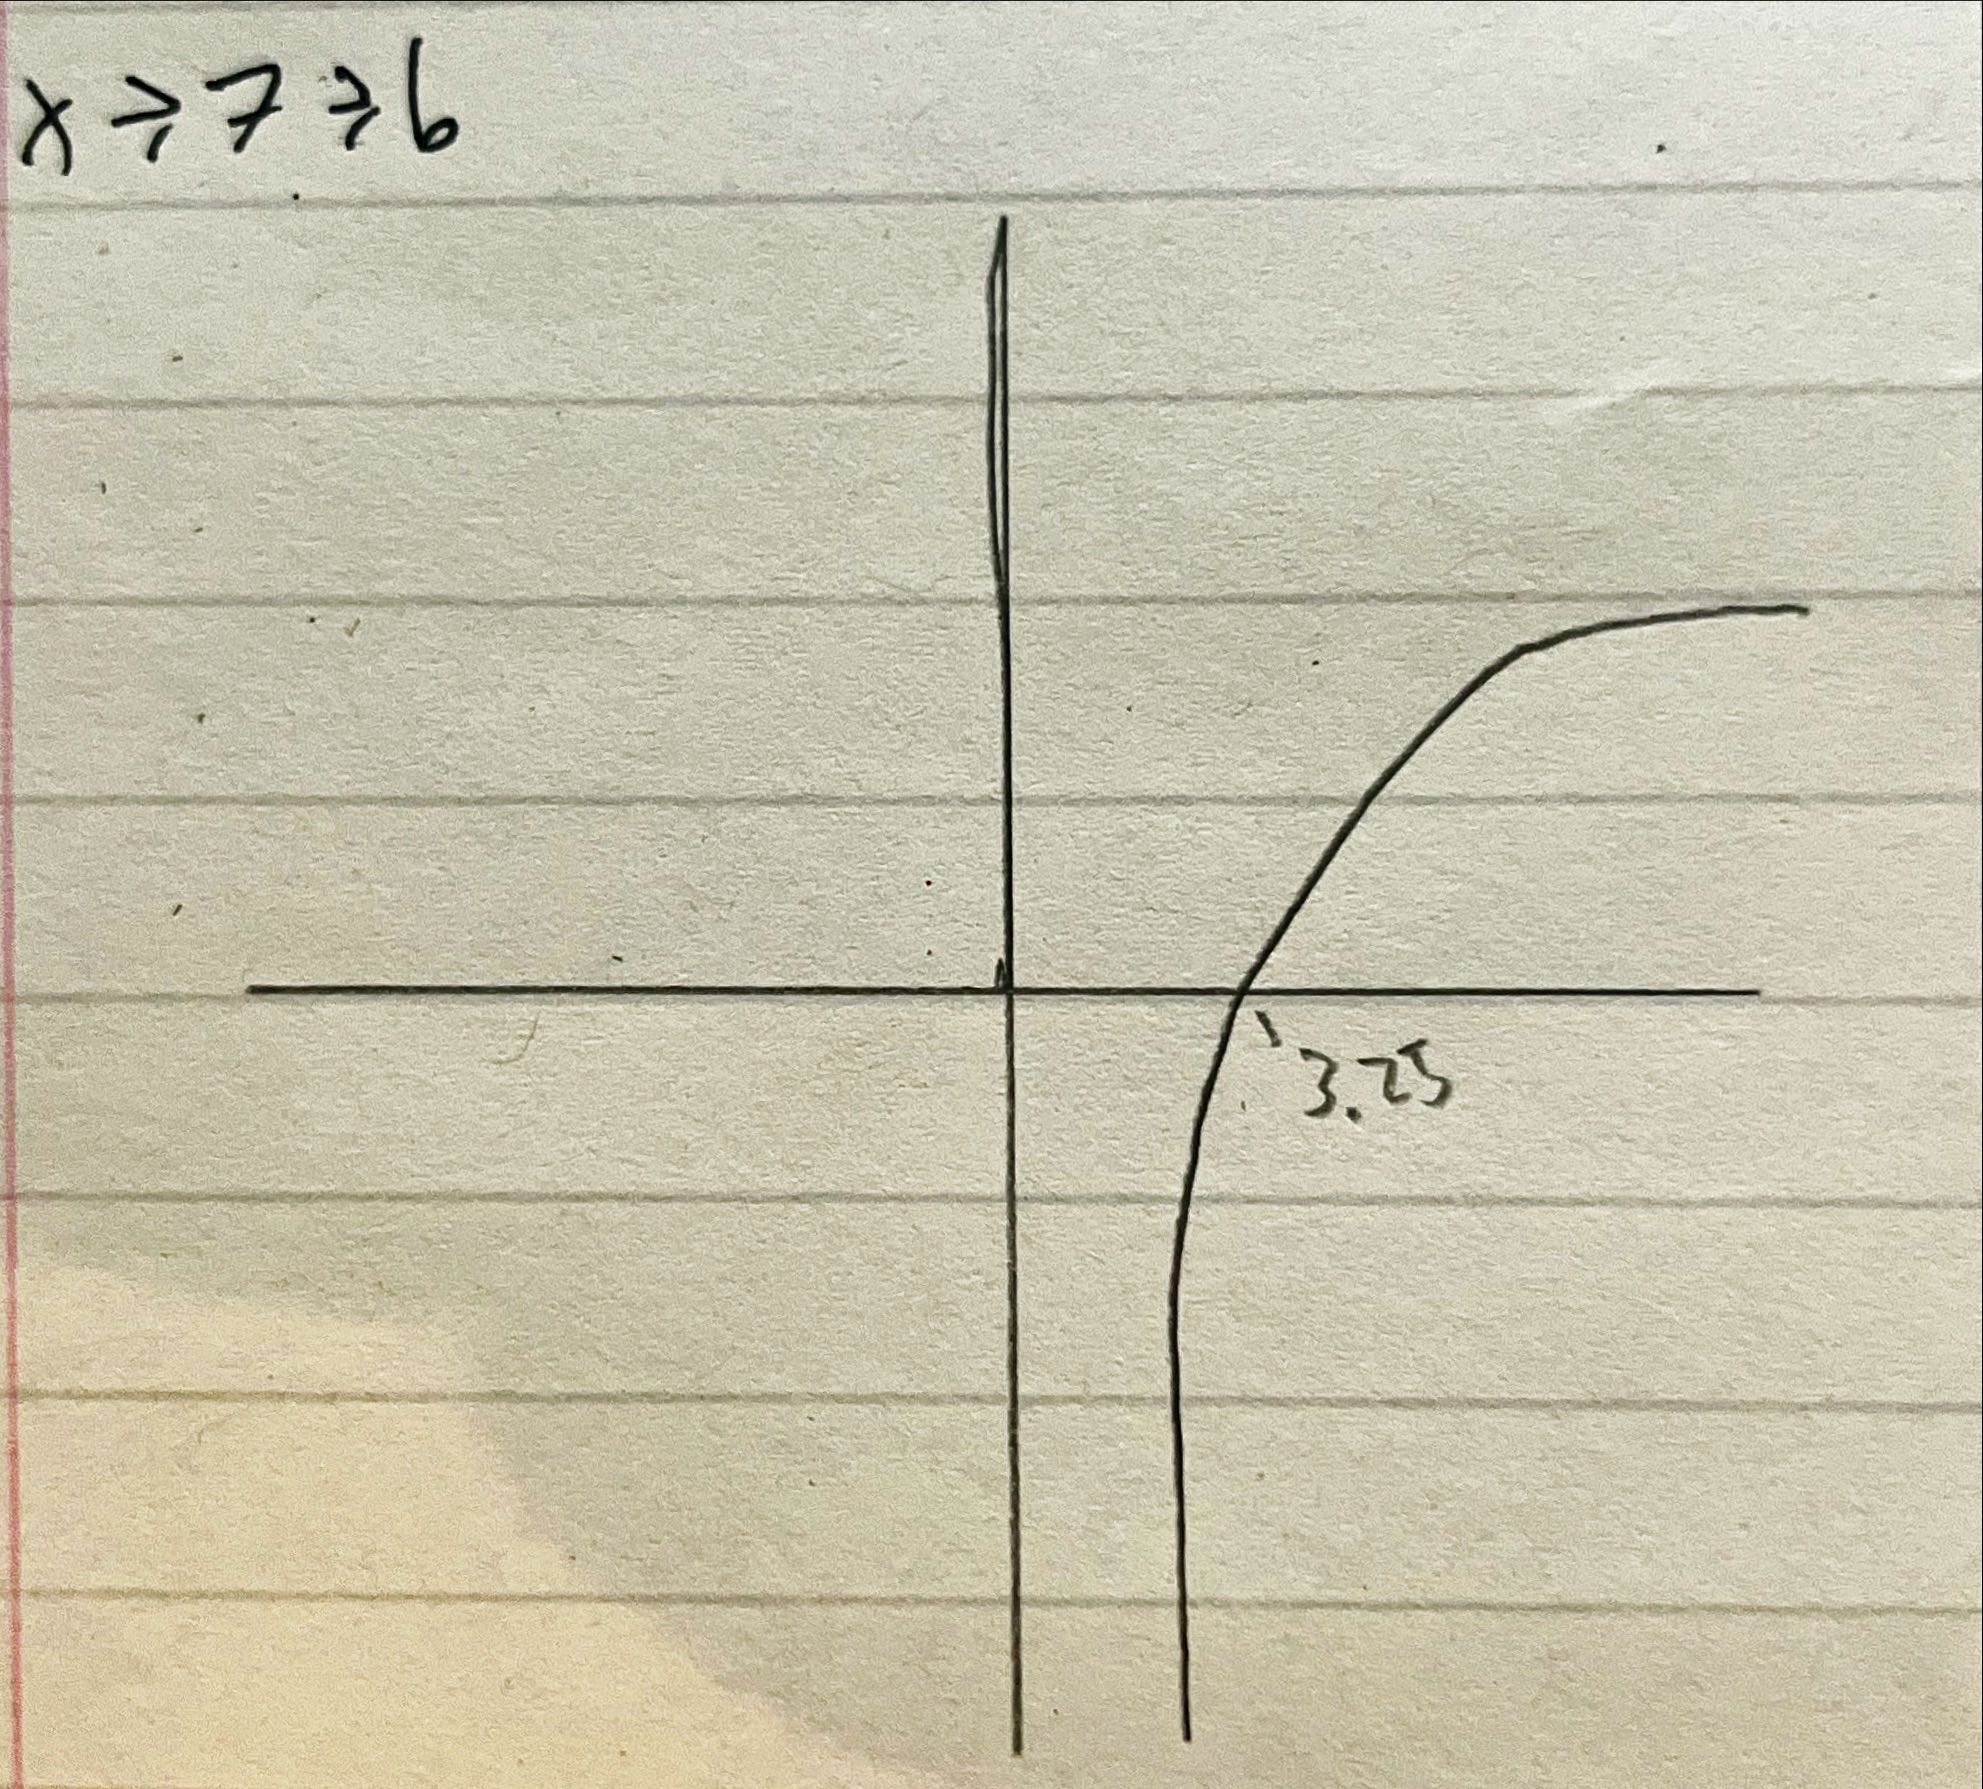
\includegraphics[width=\textwidth / 3]{x7b}
}
}

\qs{
\qsp{a}{
	\begin{multicols}{2}
		\noindent
		\begin{align*}
			v &= x \\
			v^\prime &= 1 \\
		\end{align*}
		\begin{align*}
			u &= \sqrt{x+1} \\
			u^\prime &= \frac{1}{2}(x+1)^{-\frac{1}{2}}
		\end{align*}
	\end{multicols}
	\begin{align*}
		\differen &= vu^\prime + v^\prime u \\
		&= x\frac{1}{2}(x+1)^{-\frac{1}{2}} + (x+1)^{\frac{1}{2}} \\
		&= (x+1)^{-\frac{1}{2}}\left( x\frac{1}{2} + (x+1) \right) \\
		&= (x+1)^{-\frac{1}{2}}\left( \frac{3}{2}x+1 \right) \\
		&= \frac{1}{2}(3x+2)(x+1)^{-\frac{1}{2}}
	\end{align*}
}
\qsp{b}{
	\begin{multicols}{2}
		\noindent
		\begin{align*}
			v &= x\sqrt{x+1} \\
			v^\prime &= \frac{1}{2}(3x+2)(x+1)^{-\frac{1}{2}}
		\end{align*}
		\columnbreak
		\begin{align*}
			u &= \sin 2x \\
			u^\prime &= 2\cos 2x
		\end{align*}
	\end{multicols}
	\begin{align*}
		\differen &= vu^\prime + v^\prime u \\
		&= \left( x\sqrt{x+1} \right) \left( 2\cos 2x \right) + \left( \frac{1}{2}(3x+2)(x+1)^{-\frac{1}{2}} \right) \left( \sin 2x \right) \\
		&= \left( \frac{\pi}{2}\sqrt{\frac{\pi}{2}+1} \right) \left( 2\cos \pi \right) + \left( \frac{1}{2}(3\frac{\pi}{2}+2)(\frac{\pi}{2}+1)^{-\frac{1}{2}} \right) \left( \sin \pi \right) \\
		&= -2 \left( \frac{\pi}{2}\sqrt{\frac{\pi}{2}+1} \right)
	\end{align*}
}
}

\end{document}
